%%%%%%%%%%%%%%%%%%%%%%%%%%%%%%%%%%%%%%%%%
% Beamer Presentation
% LaTeX Template
% Version 1.0 (10/11/12)
%
% This template has been downloaded from:
% http://www.LaTeXTemplates.com
%
% License:
% CC BY-NC-SA 3.0 (http://creativecommons.org/licenses/by-nc-sa/3.0/)
%
%%%%%%%%%%%%%%%%%%%%%%%%%%%%%%%%%%%%%%%%%

%----------------------------------------------------------------------------------------
%    PACKAGES AND THEMES
%----------------------------------------------------------------------------------------

\documentclass[usenames,dvipsnames]{beamer}
\usepackage{animate}
\usepackage{float}
\usepackage{bm}
\usepackage{mathtools}
\usepackage{extarrows}

\usepackage[T1]{fontenc}
\usepackage{beramono}
\usepackage{listings}
\usepackage{xcolor}

%%
%% Julia definition (c) 2014 Jubobs
%%
\lstdefinelanguage{Julia}%
  {morekeywords={abstract,break,case,catch,const,continue,do,else,elseif,%
      end,export,false,for,function,immutable,import,importall,if,in,%
      macro,module,otherwise,quote,return,switch,true,try,type,typealias,%
      using,while},%
   sensitive=true,%
   morecomment=[l]\#,%
   morecomment=[n]{\#=}{=\#},%
   morestring=[s]{"}{"},%
   morestring=[m]{'}{'},%
}[keywords,comments,strings]%

\lstset{%
    language         = Julia,
    basicstyle       = \ttfamily,
    keywordstyle     = \bfseries\color{blue},
    stringstyle      = \color{magenta},
    commentstyle     = \color{ForestGreen},
    showstringspaces = false,
}
\newcommand{\ChoL}{\mathsf{L}}
\newcommand{\bx}{\mathbf{x}}
\newcommand{\ii}{\mathrm{i}}
\newcommand{\bxi}{\bm{\xi}}
\newcommand{\bmu}{\bm{\mu}}
\newcommand{\bb}{\mathbf{b}}
\newcommand{\bA}{\mathbf{A}}
\newcommand{\bJ}{\mathbf{J}}
\newcommand{\bB}{\mathbf{B}}
\newcommand{\bM}{\mathbf{M}}

\newcommand{\by}{\mathbf{y}}
\newcommand{\bw}{\mathbf{w}}

\newcommand{\bX}{\mathbf{X}}
\newcommand{\bY}{\mathbf{Y}}
\newcommand{\bs}{\mathbf{s}}
\newcommand{\sign}{\mathrm{sign}}
\newcommand{\bt}[0]{\bm{\theta}}
\newcommand{\bc}{\mathbf{c}}
\newcommand{\bzero}{\mathbf{0}}
\renewcommand{\bf}{\mathbf{f}}
\newcommand{\bu}{\mathbf{u}}
\newcommand{\bv}[0]{\mathbf{v}}

\mode<presentation> {

% The Beamer class comes with a number of default slide themes
% which change the colors and layouts of slides. Below this is a list
% of all the themes, uncomment each in turn to see what they look like.

%\usetheme{default}
%\usetheme{AnnArbor}
%\usetheme{Antibes}
%\usetheme{Bergen}
%\usetheme{Berkeley}
%\usetheme{Berlin}
%\usetheme{Boadilla}
%\usetheme{CambridgeUS}
%\usetheme{Copenhagen}
%\usetheme{Darmstadt}
%\usetheme{Dresden}
%\usetheme{Frankfurt}
%\usetheme{Goettingen}
%\usetheme{Hannover}
%\usetheme{Ilmenau}
%\usetheme{JuanLesPins}
%\usetheme{Luebeck}
\usetheme{Madrid}
%\usetheme{Malmoe}
%\usetheme{Marburg}
%\usetheme{Montpellier}
%\usetheme{PaloAlto}
%\usetheme{Pittsburgh}
%\usetheme{Rochester}
%\usetheme{Singapore}
%\usetheme{Szeged}
%\usetheme{Warsaw}


% As well as themes, the Beamer class has a number of color themes
% for any slide theme. Uncomment each of these in turn to see how it
% changes the colors of your current slide theme.

%\usecolortheme{albatross}
\usecolortheme{beaver}
%\usecolortheme{beetle}
%\usecolortheme{crane}
%\usecolortheme{dolphin}
%\usecolortheme{dove}
%\usecolortheme{fly}
%\usecolortheme{lily}
%\usecolortheme{orchid}
%\usecolortheme{rose}
%\usecolortheme{seagull}
%\usecolortheme{seahorse}
%\usecolortheme{whale}
%\usecolortheme{wolverine}

%\setbeamertemplate{footline} % To remove the footer line in all slides uncomment this line
%\setbeamertemplate{footline}[page number] % To replace the footer line in all slides with a simple slide count uncomment this line

%\setbeamertemplate{navigation symbols}{} % To remove the navigation symbols from the bottom of all slides uncomment this line
}
\usepackage{booktabs}
\usepackage{makecell}

\usepackage{soul}
\newcommand{\red}[1]{\textcolor{red}{#1}}
%
%\usepackage{graphicx} % Allows including images
%\usepackage{booktabs} % Allows the use of \toprule, \midrule and \bottomrule in tables
%
%
%\usepackage{amsthm}
%
%\usepackage{todonotes}
%\usepackage{floatrow}
%
%\usepackage{pgfplots,algorithmic,algorithm}
\usepackage{algorithmicx}
\usepackage{algpseudocode}
%\usepackage[toc,page]{appendix}
%\usepackage{float}
%\usepackage{booktabs}
%\usepackage{bm}
%
%\theoremstyle{definition}
%
\newcommand{\RR}[0]{\mathbb{R}}
%
%\newcommand{\bx}{\mathbf{x}}
%\newcommand{\ii}{\mathrm{i}}
%\newcommand{\bxi}{\bm{\xi}}
%\newcommand{\bmu}{\bm{\mu}}
%\newcommand{\bb}{\mathbf{b}}
%\newcommand{\bA}{\mathbf{A}}
%\newcommand{\bJ}{\mathbf{J}}
%\newcommand{\bB}{\mathbf{B}}
%\newcommand{\bM}{\mathbf{M}}
%\newcommand{\bF}{\mathbf{F}}
%
%\newcommand{\by}{\mathbf{y}}
%\newcommand{\bw}{\mathbf{w}}
%\newcommand{\bn}{\mathbf{n}}
%
%\newcommand{\bX}{\mathbf{X}}
%\newcommand{\bY}{\mathbf{Y}}
%\newcommand{\bs}{\mathbf{s}}
%\newcommand{\sign}{\mathrm{sign}}
%\newcommand{\bt}[0]{\bm{\theta}}
%\newcommand{\bc}{\mathbf{c}}
%\newcommand{\bzero}{\mathbf{0}}
%\renewcommand{\bf}{\mathbf{f}}
%\newcommand{\bu}{\mathbf{u}}
%\newcommand{\bv}[0]{\mathbf{v}}

\AtBeginSection[]
{
   \begin{frame}
       \frametitle{Outline}
       \tableofcontents[currentsection]
   \end{frame}
}

%----------------------------------------------------------------------------------------
%    TITLE PAGE
%----------------------------------------------------------------------------------------
\usepackage{bm}
\newcommand*{\TakeFourierOrnament}[1]{{%
\fontencoding{U}\fontfamily{futs}\selectfont\char#1}}
\newcommand*{\danger}{\TakeFourierOrnament{66}}

\title[ML for Computational Engineering]{ADCME \\ Machine Learning for Computational Engineering} % The short title appears at the bottom of every slide, the full title is only on the title page

\author[ADCME]{Kailai Xu and Eric Darve\\\url{https://github.com/kailaix/ADCME.jl}} % Your name
%\institute[] % Your institution as it will appear on the bottom of every slide, may be shorthand to save space
%{
%%ICME, Stanford University \\ % Your institution for the title page
%%\medskip
%%\textit{kailaix@stanford.edu}\quad \textit{darve@stanford.edu} % Your email address
%}
\date{}% Date, can be changed to a custom date
% Mathematics of PDEs


\begin{document}

\usebackgroundtemplate{%
\begin{picture}(0,250)
\centering
	{{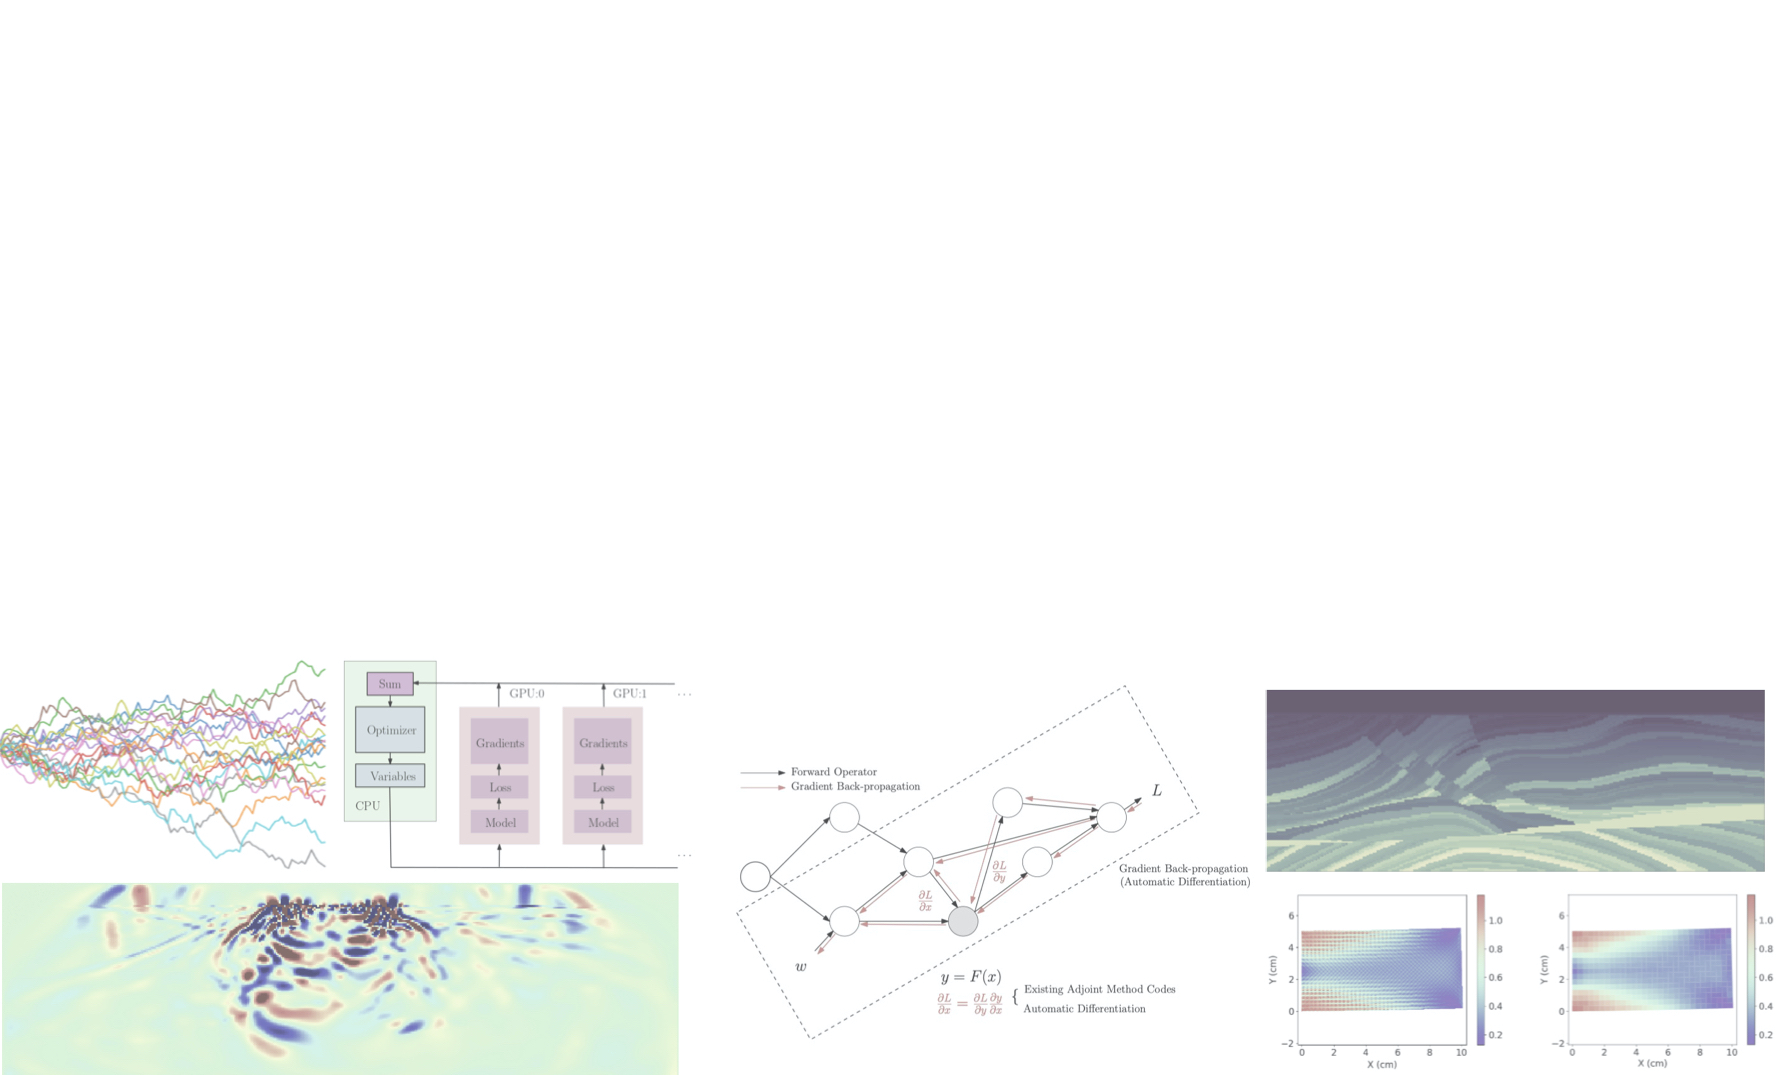
\includegraphics[width=1.0\paperwidth]{figures/background}}}
\end{picture}
  } 
%\usebackgroundtemplate{%
%  \includegraphics[width=\paperwidth,height=\paperheight]{figures/back}} 
\begin{frame}

\titlepage % Print the title page as the first slide

%dfa
\end{frame}
\usebackgroundtemplate{}

\begin{frame}
	\frametitle{Inverse Modeling}
	\begin{figure}
	\centering
  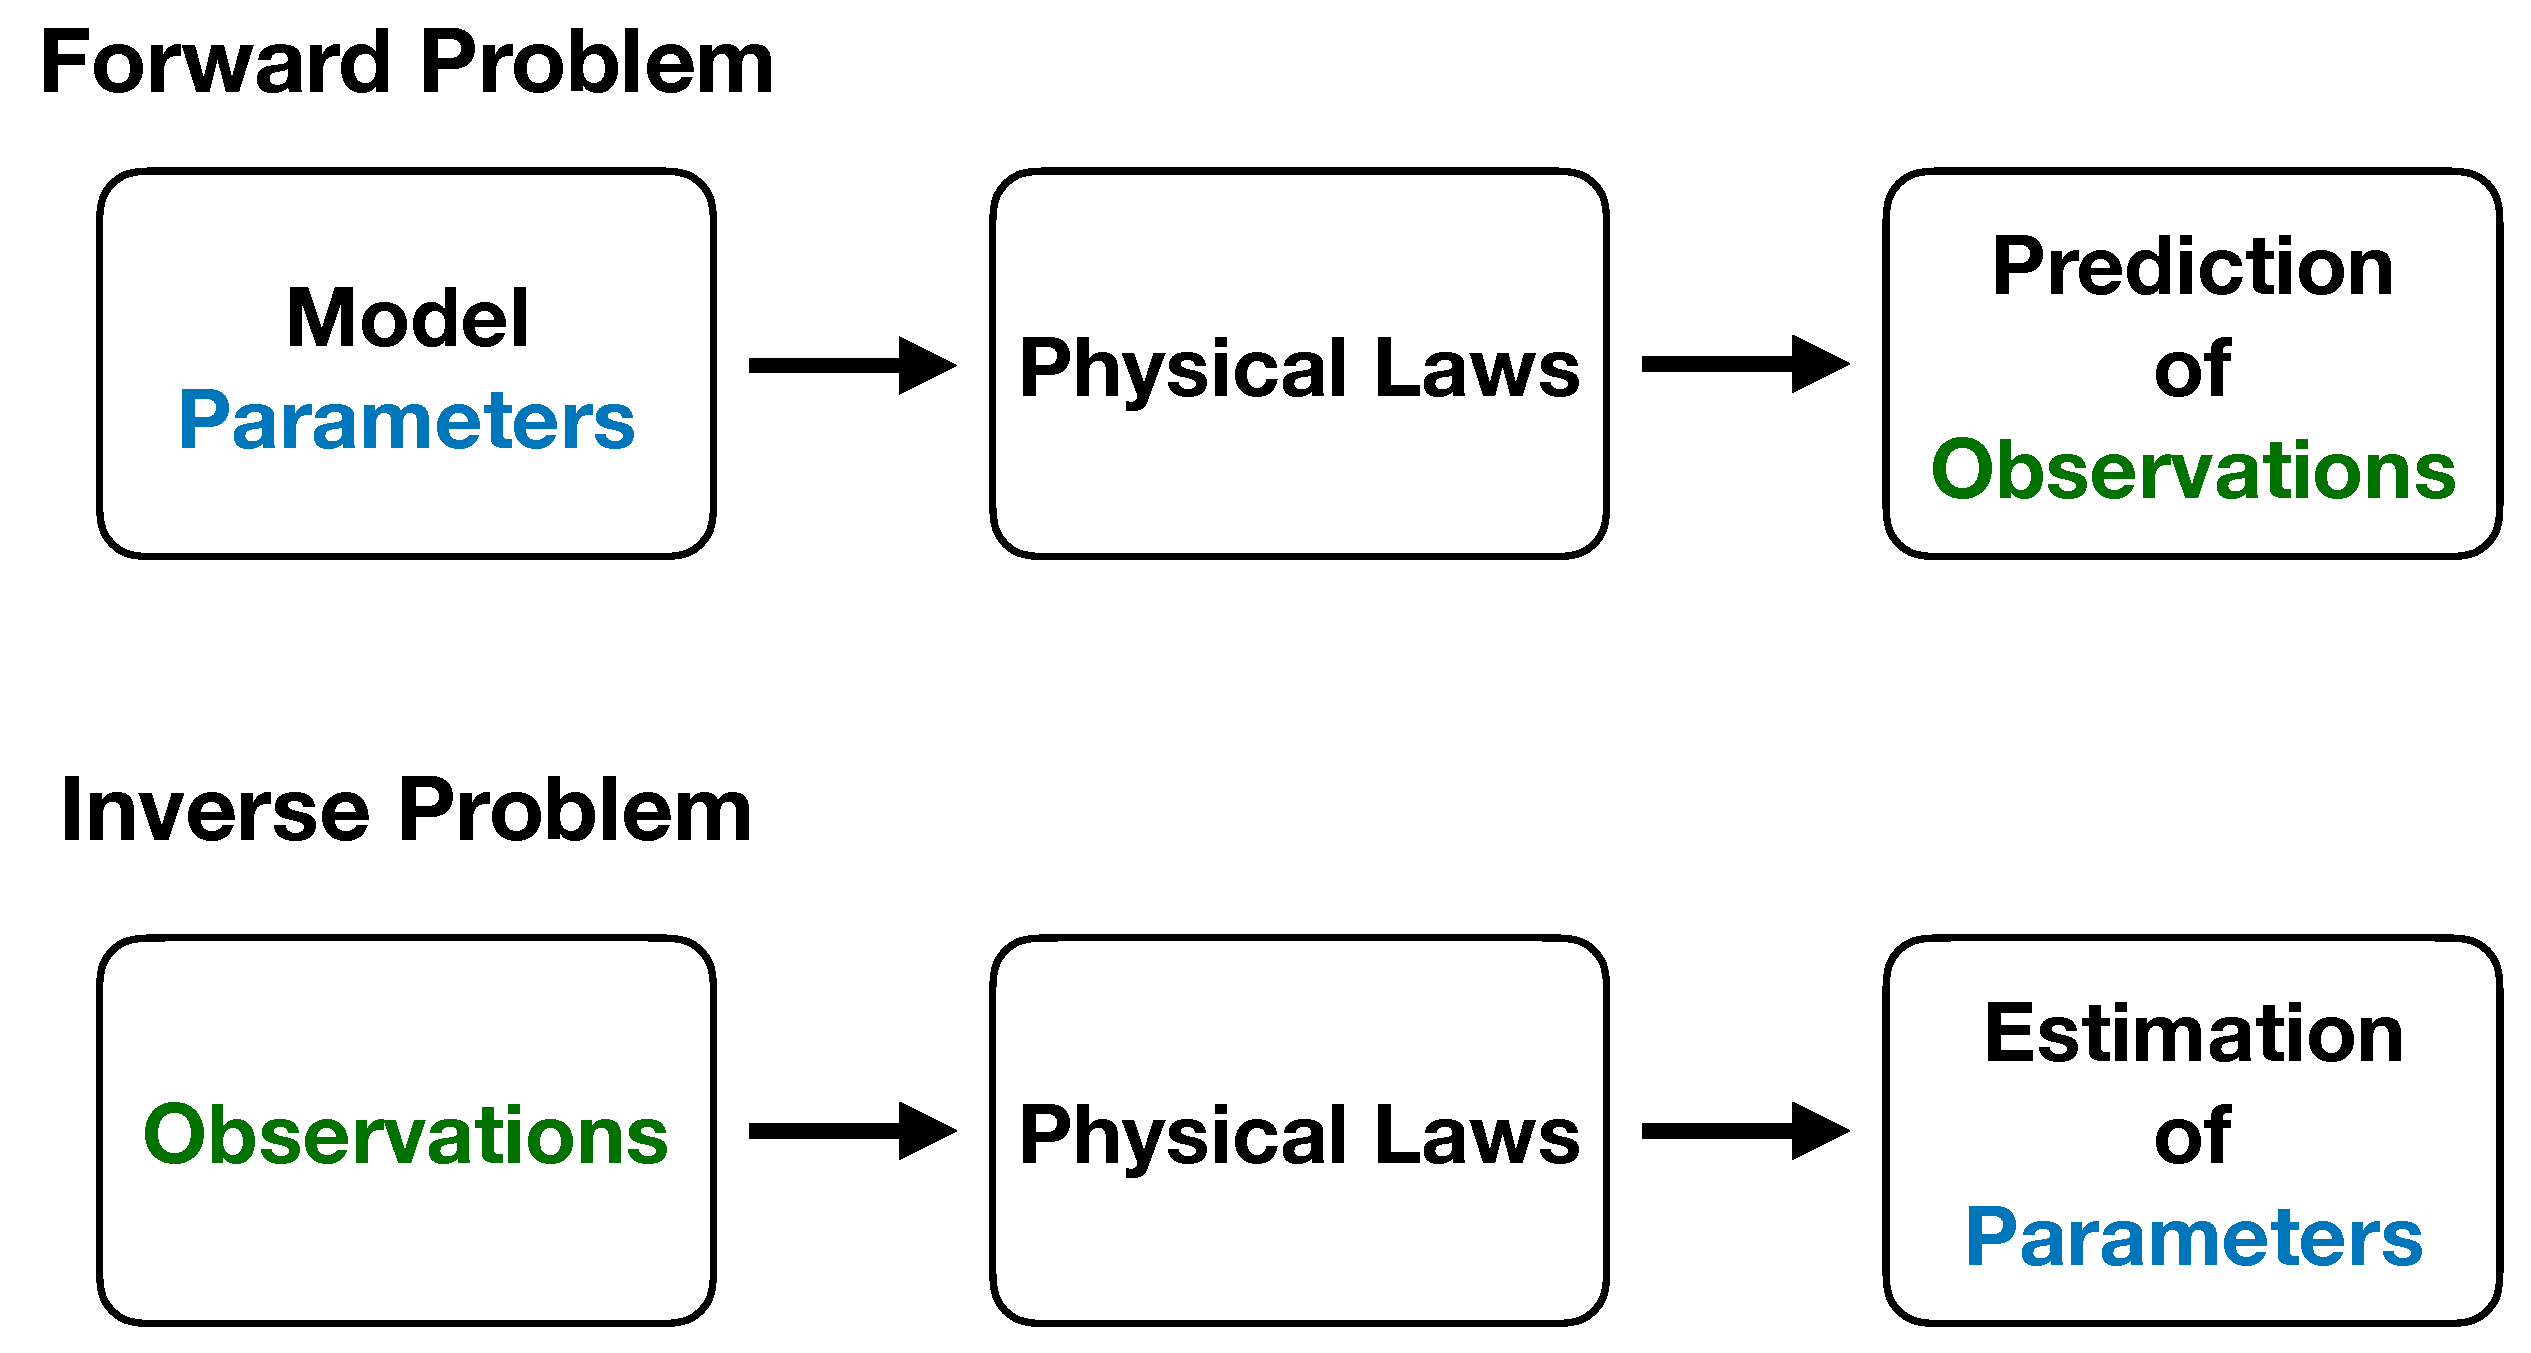
\includegraphics[width=1.0\textwidth]{figures/inverse3}
\end{figure}
\end{frame}

\begin{frame}
	\frametitle{Function Inverse Problem}
	
	\begin{equation*}
		\min_{\textcolor{red}{f}} L_h(u_h) \quad \mathrm{s.t.}\; F_h(\textcolor{red}{f}, u_h) = 0
	\end{equation*}
	
	What if the unknown is a \textcolor{red}{function} instead of a set of parameters?
\begin{itemize}
	\item Koopman operator in dynamical systems.
	\item Constitutive relations in solid mechanics. 
	\item Turbulent closure relations in fluid mechanics.
	\item ...
\end{itemize}

The candidate solution space is \textcolor{red}{infinite dimensional}.

\end{frame}

\begin{frame}
	\frametitle{Physics Based Machine Learning}
	$$\min_{\theta} L_h(u_h) \quad \mathrm{s.t.}\;F_h(\textcolor{red}{NN_\theta}, u_h) = 0$$
	\vspace{-0.5cm}
	\begin{itemize}
		\item Deep neural networks exhibit capability of approximating high dimensional and complicated functions. 
		\item \textbf{Physics based machine learning}: \textcolor{red}{the unknown function is approximated by a deep neural network, and the physical constraints are enforced by numerical schemes}.
		\item \textcolor{red}{Satisfy the physics to the largest extent}.
	\end{itemize}
	\begin{figure}[hbt]
  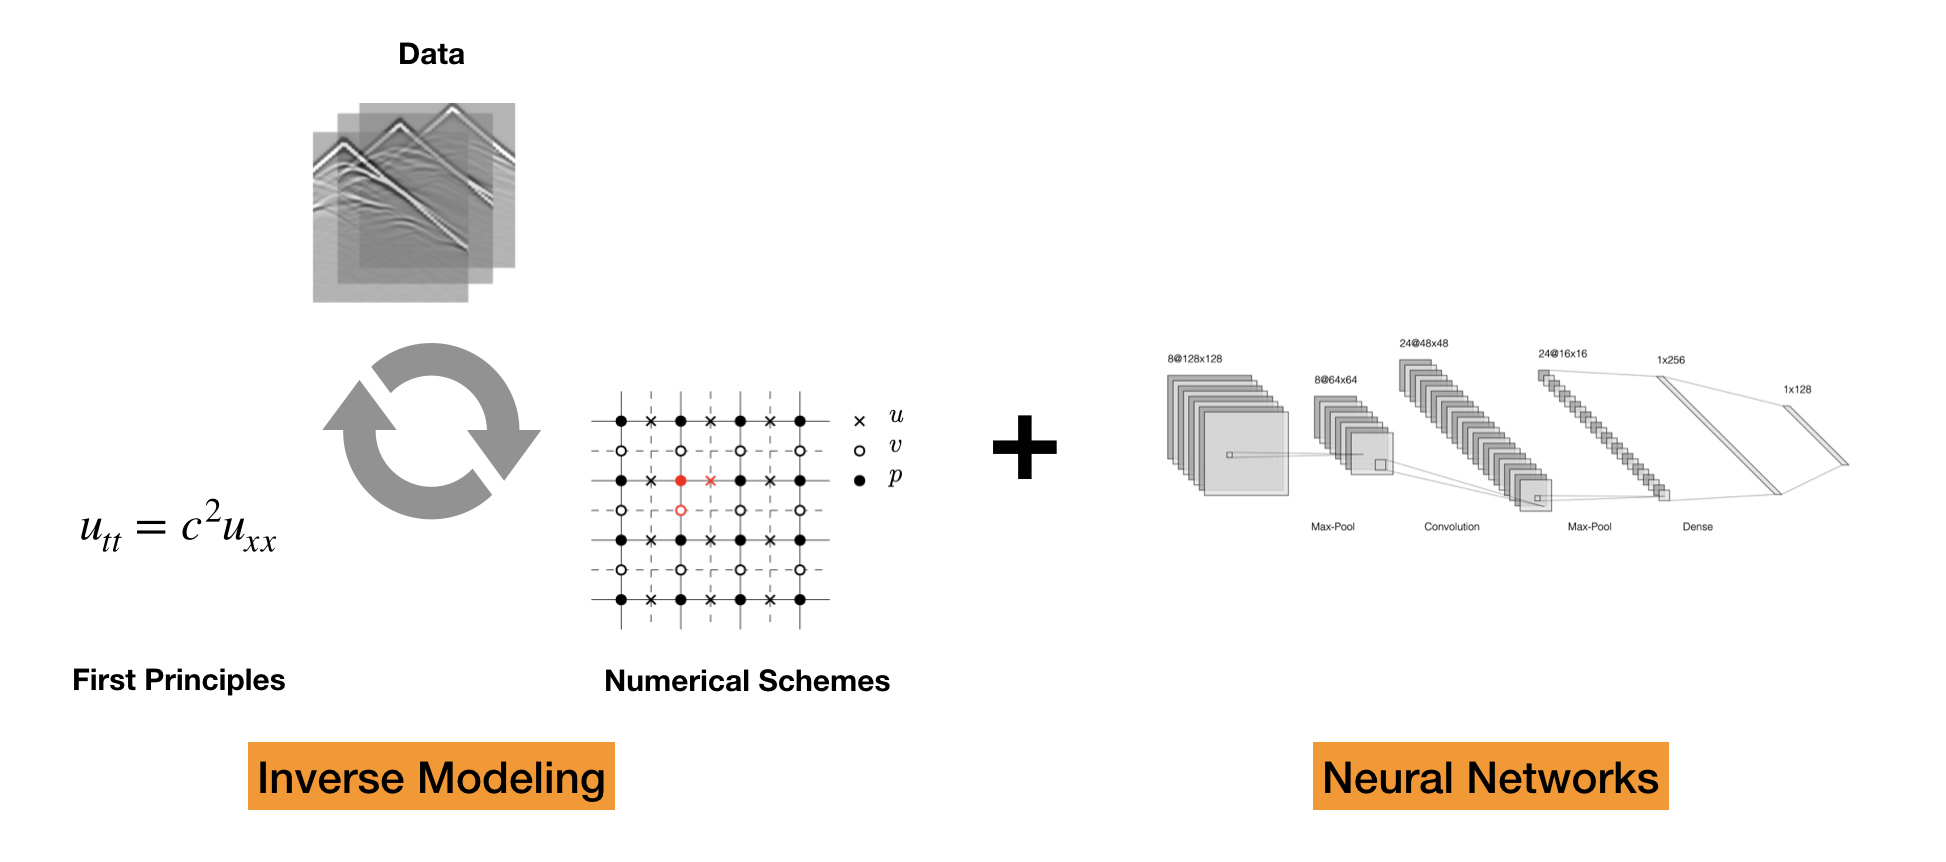
\includegraphics[width=0.75\textwidth]{figures/physics_based_machine_learning.png}
\end{figure}
\end{frame}




\begin{frame}
	\frametitle{Gradient Based Optimization}
	\begin{equation}\label{equ:opt}
	\min_{\theta} L_h(u_h) \quad \mathrm{s.t.}\; F_h(\theta, u_h) = 0
	\end{equation}
	
	\begin{itemize}
		\item We can now apply a gradient-based optimization method to (\ref{equ:opt}).
		\item The key is to \textcolor{red}{calculate the gradient descent direction} $g^k$
		$$\theta^{k+1} \gets \theta^k - \alpha g^k$$ 
	\end{itemize}
	
	\begin{figure}[hbt]
		\centering
		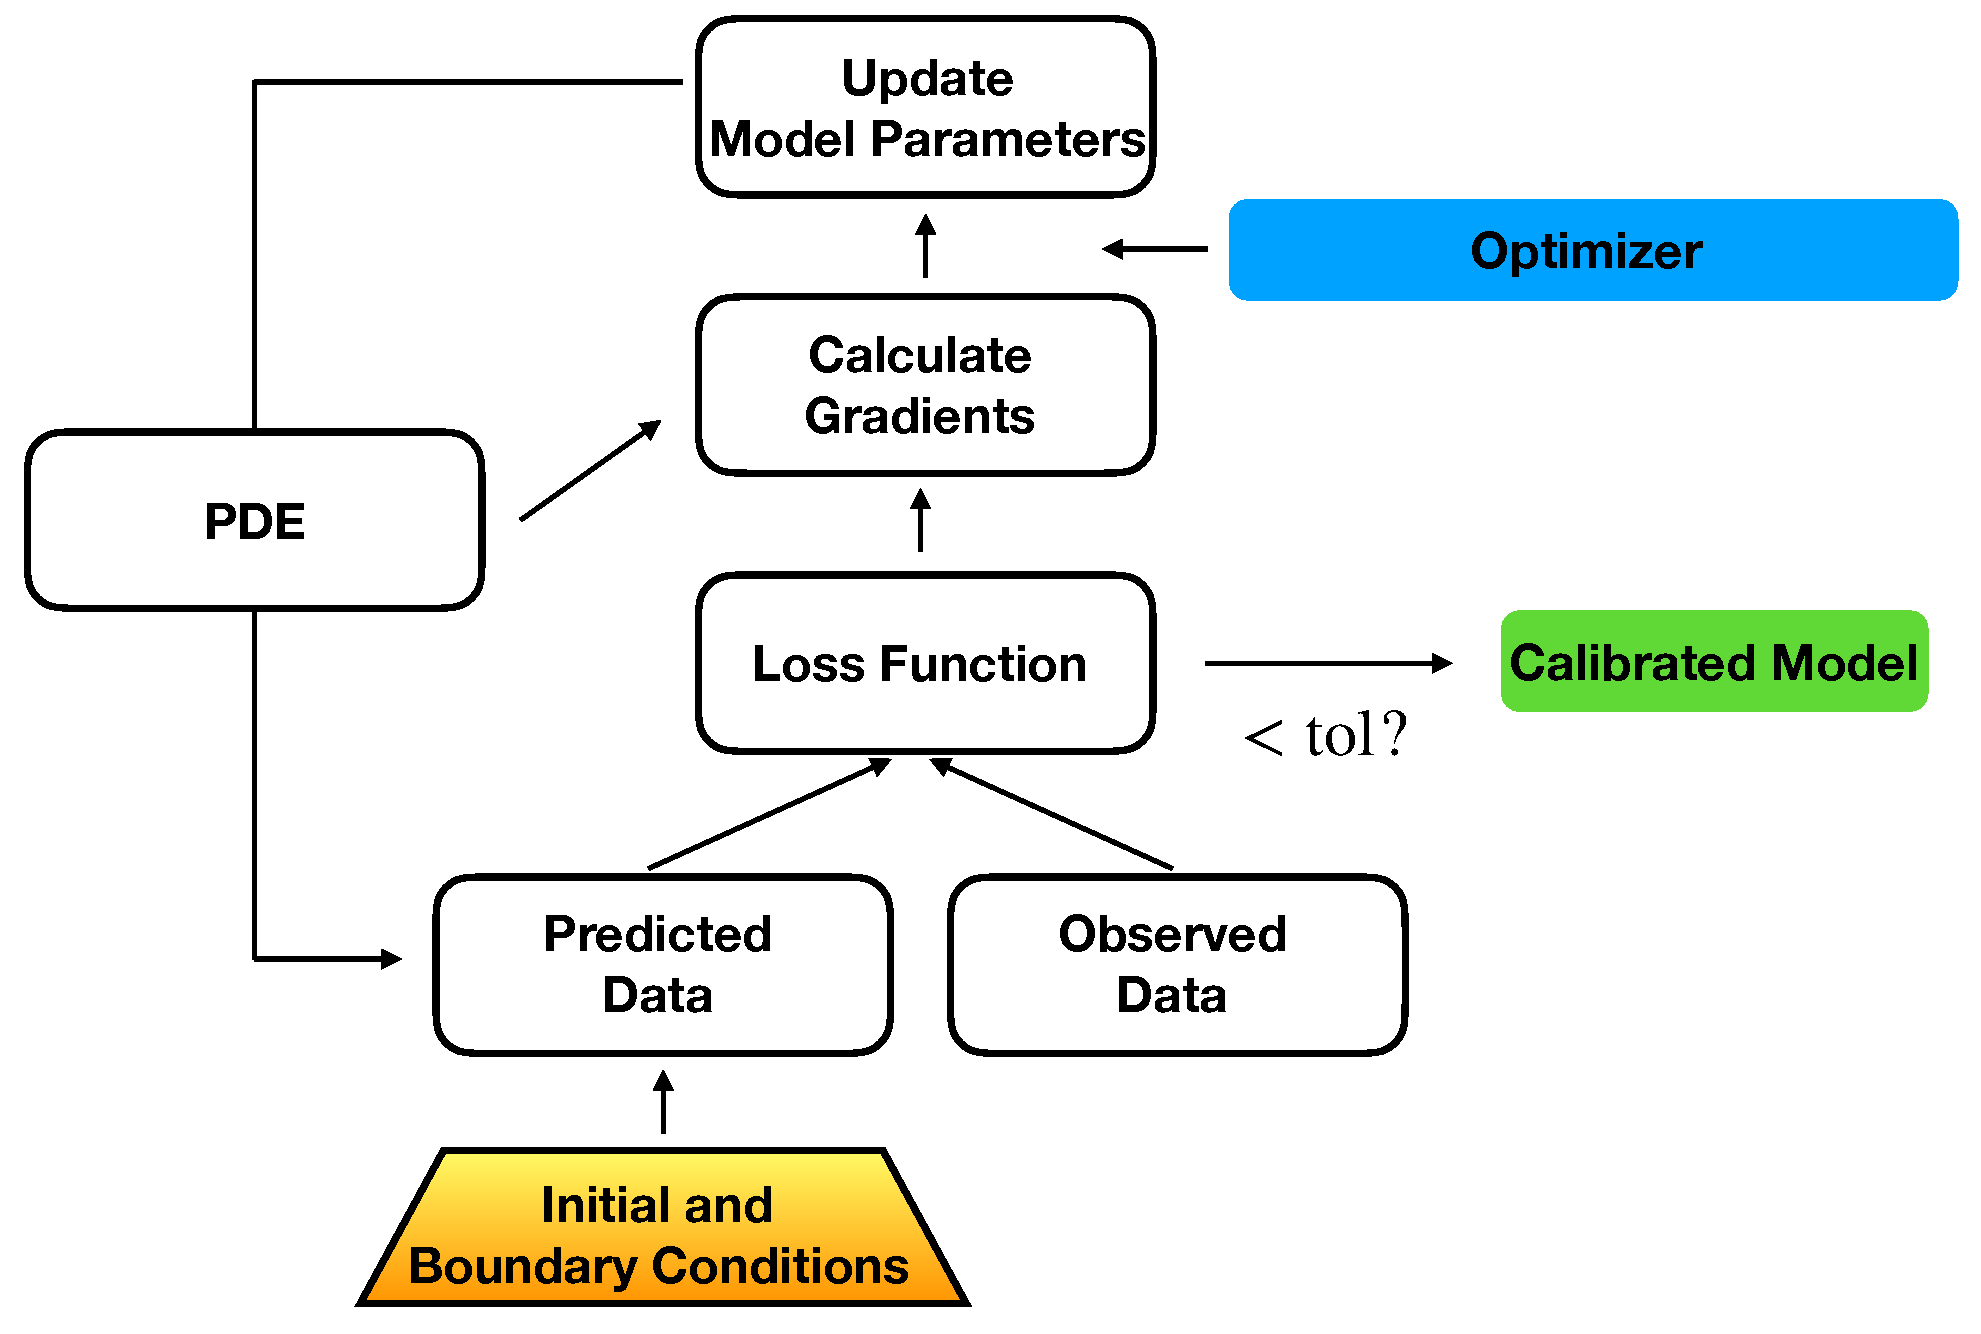
\includegraphics[width=0.6\textwidth]{figures/im.pdf}
	\end{figure}
	
\end{frame}




\begin{frame}
	\frametitle{Automatic Differentiation}
	The fact that bridges the \textcolor{red}{technical} gap between machine learning and inverse modeling:
	\begin{itemize}
		\item Deep learning (and many other machine learning techniques) and numerical schemes share the same computational model: composition of individual operators. 
	\end{itemize}
	
	
	\begin{minipage}[t]{0.4\textwidth}
		
		\
		
		
		
		\begin{center}
			\textcolor{red}{Mathematical Fact}
			
			\
			
			Back-propagation 
			
			$||$
			
			Reverse-mode
			
			Automatic Differentiation 
			
			$||$
			
			Discrete 
			
			Adjoint-State Method
		\end{center}
	\end{minipage}~
	\begin{minipage}[t]{0.6\textwidth}
		\begin{figure}[hbt]
			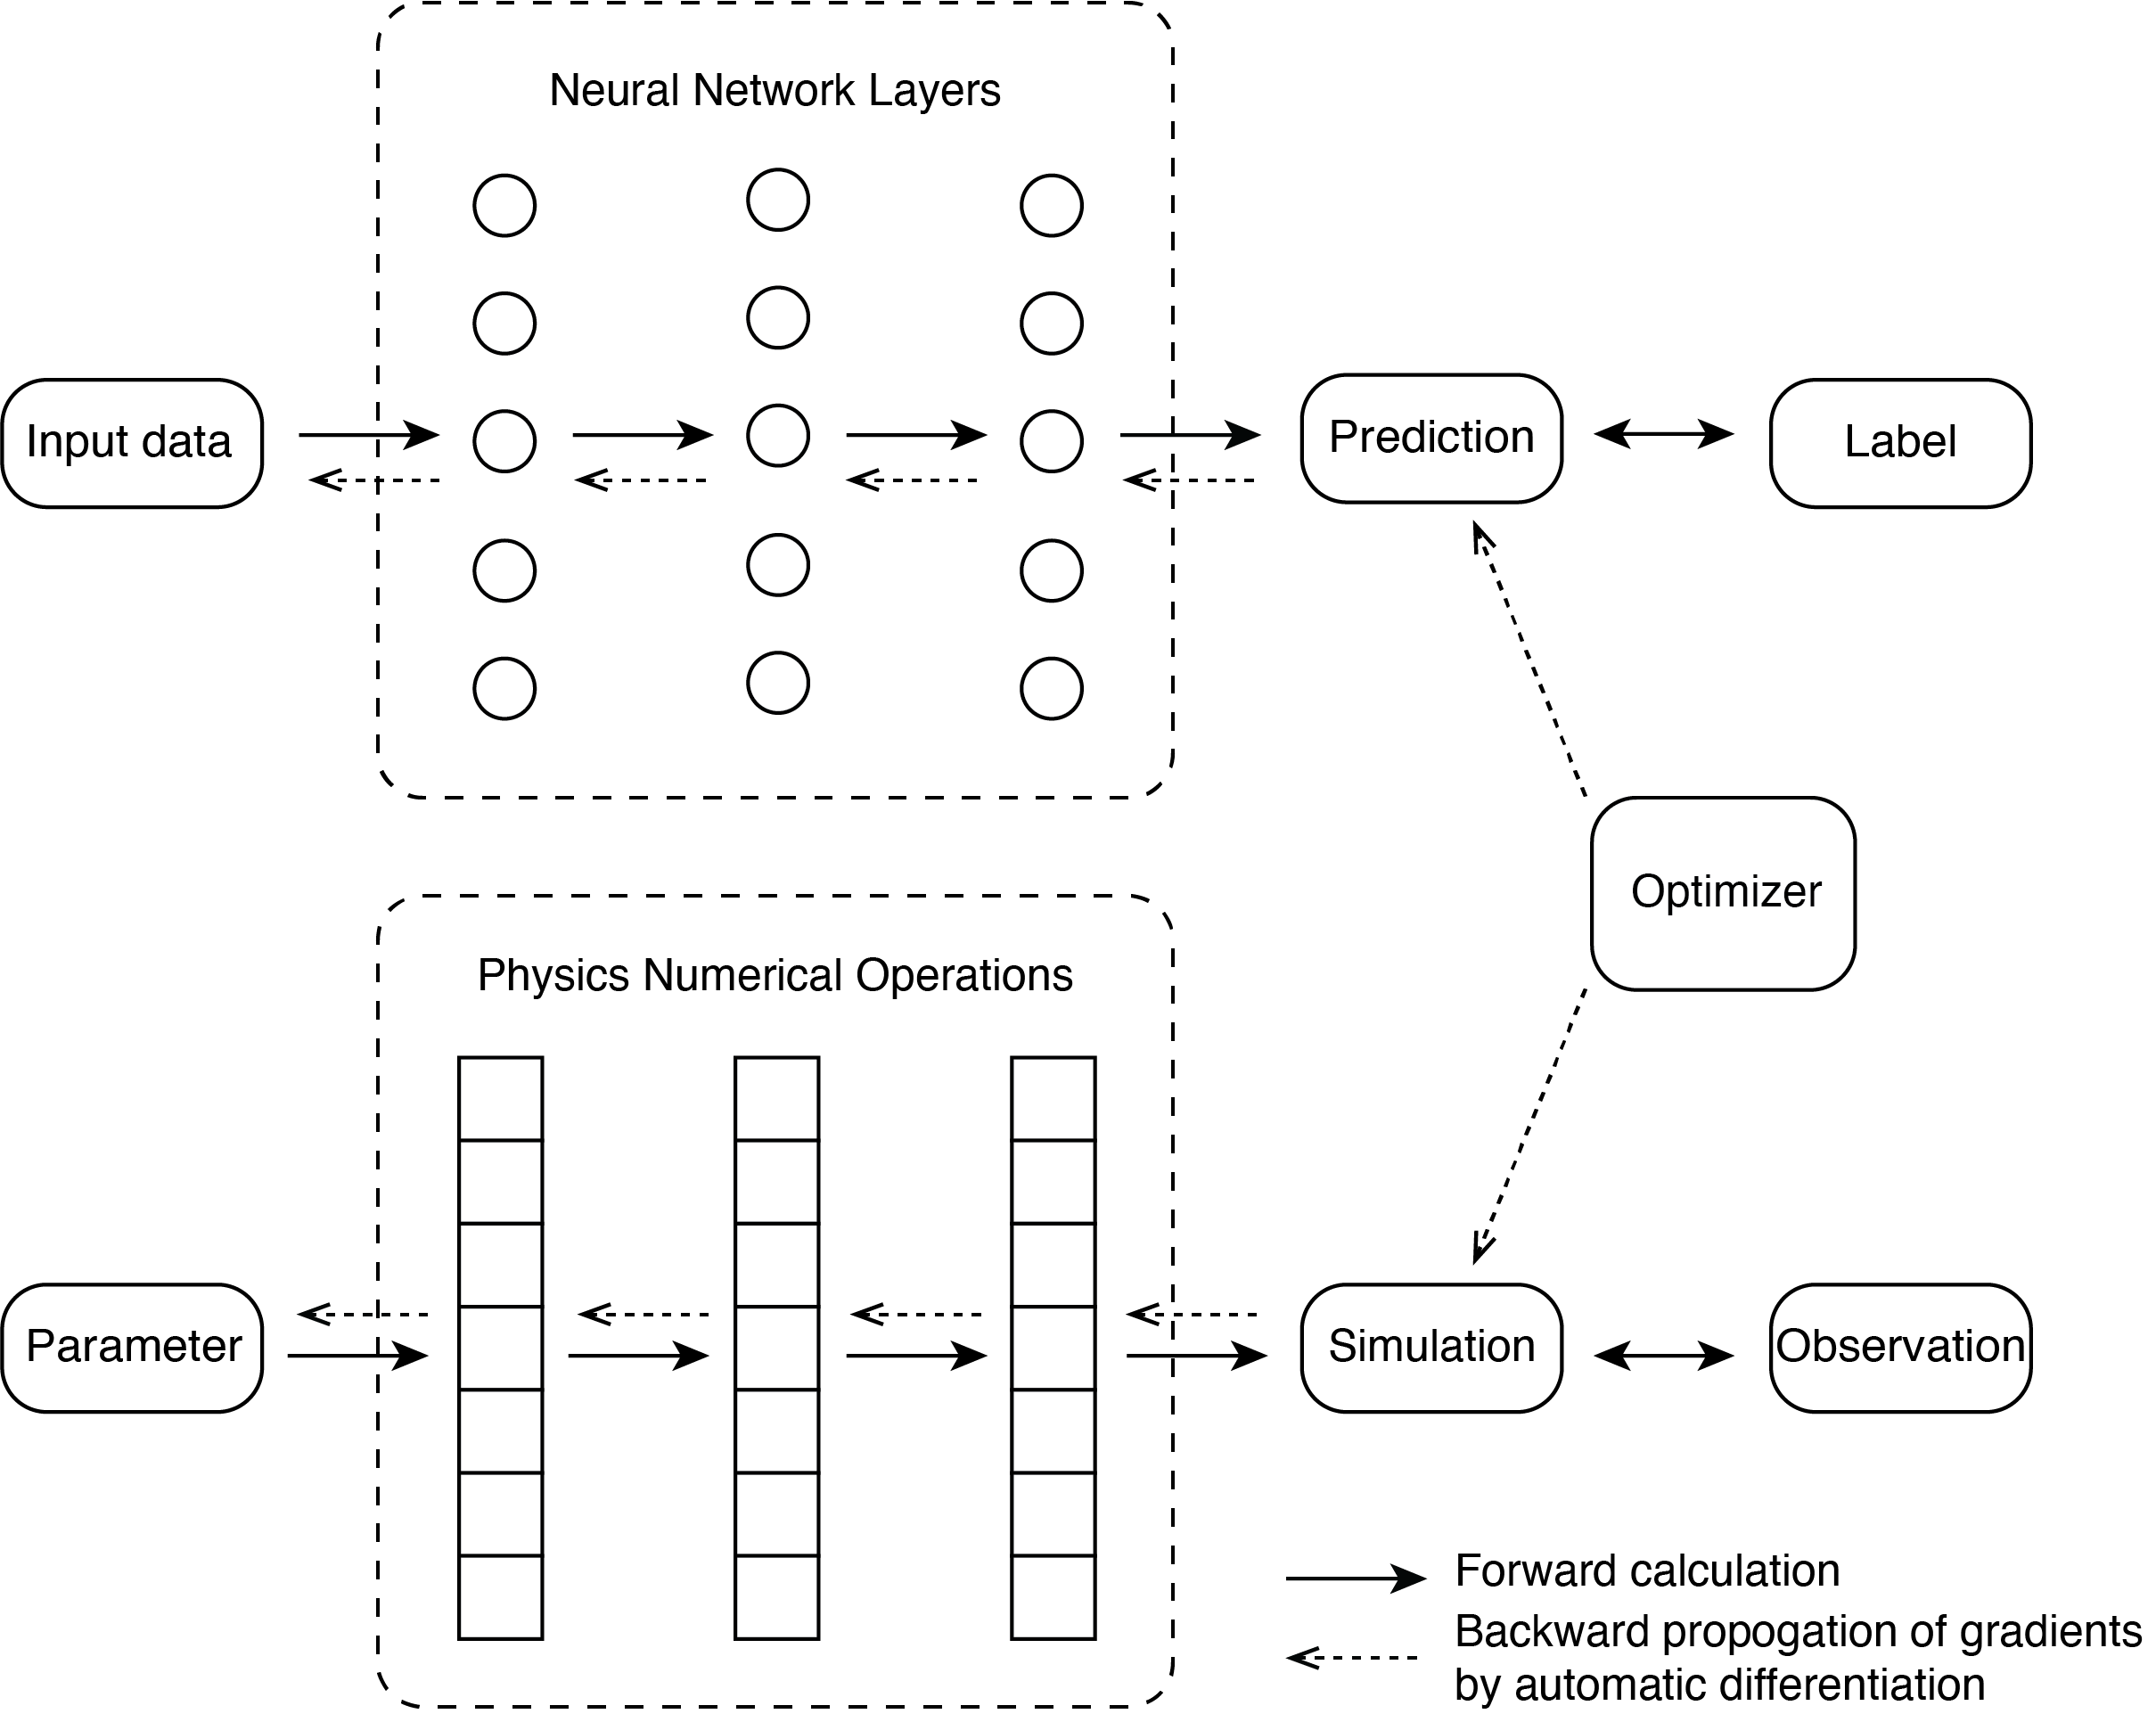
\includegraphics[width=0.8\textwidth]{figures/compare-NN-PDE.png}
		\end{figure}
	\end{minipage}
	
\end{frame}

\begin{frame}
	\frametitle{Computational Graph for Numerical Schemes}
	
	\begin{itemize}
		\item To leverage automatic differentiation for inverse modeling, we need to express the numerical schemes in the ``AD language'': computational graph. 
		\item No matter how complicated a numerical scheme is, it can be decomposed into a collection of operators that are interlinked via state variable dependencies. 
	\end{itemize}
	
	\begin{figure}[hbt]
		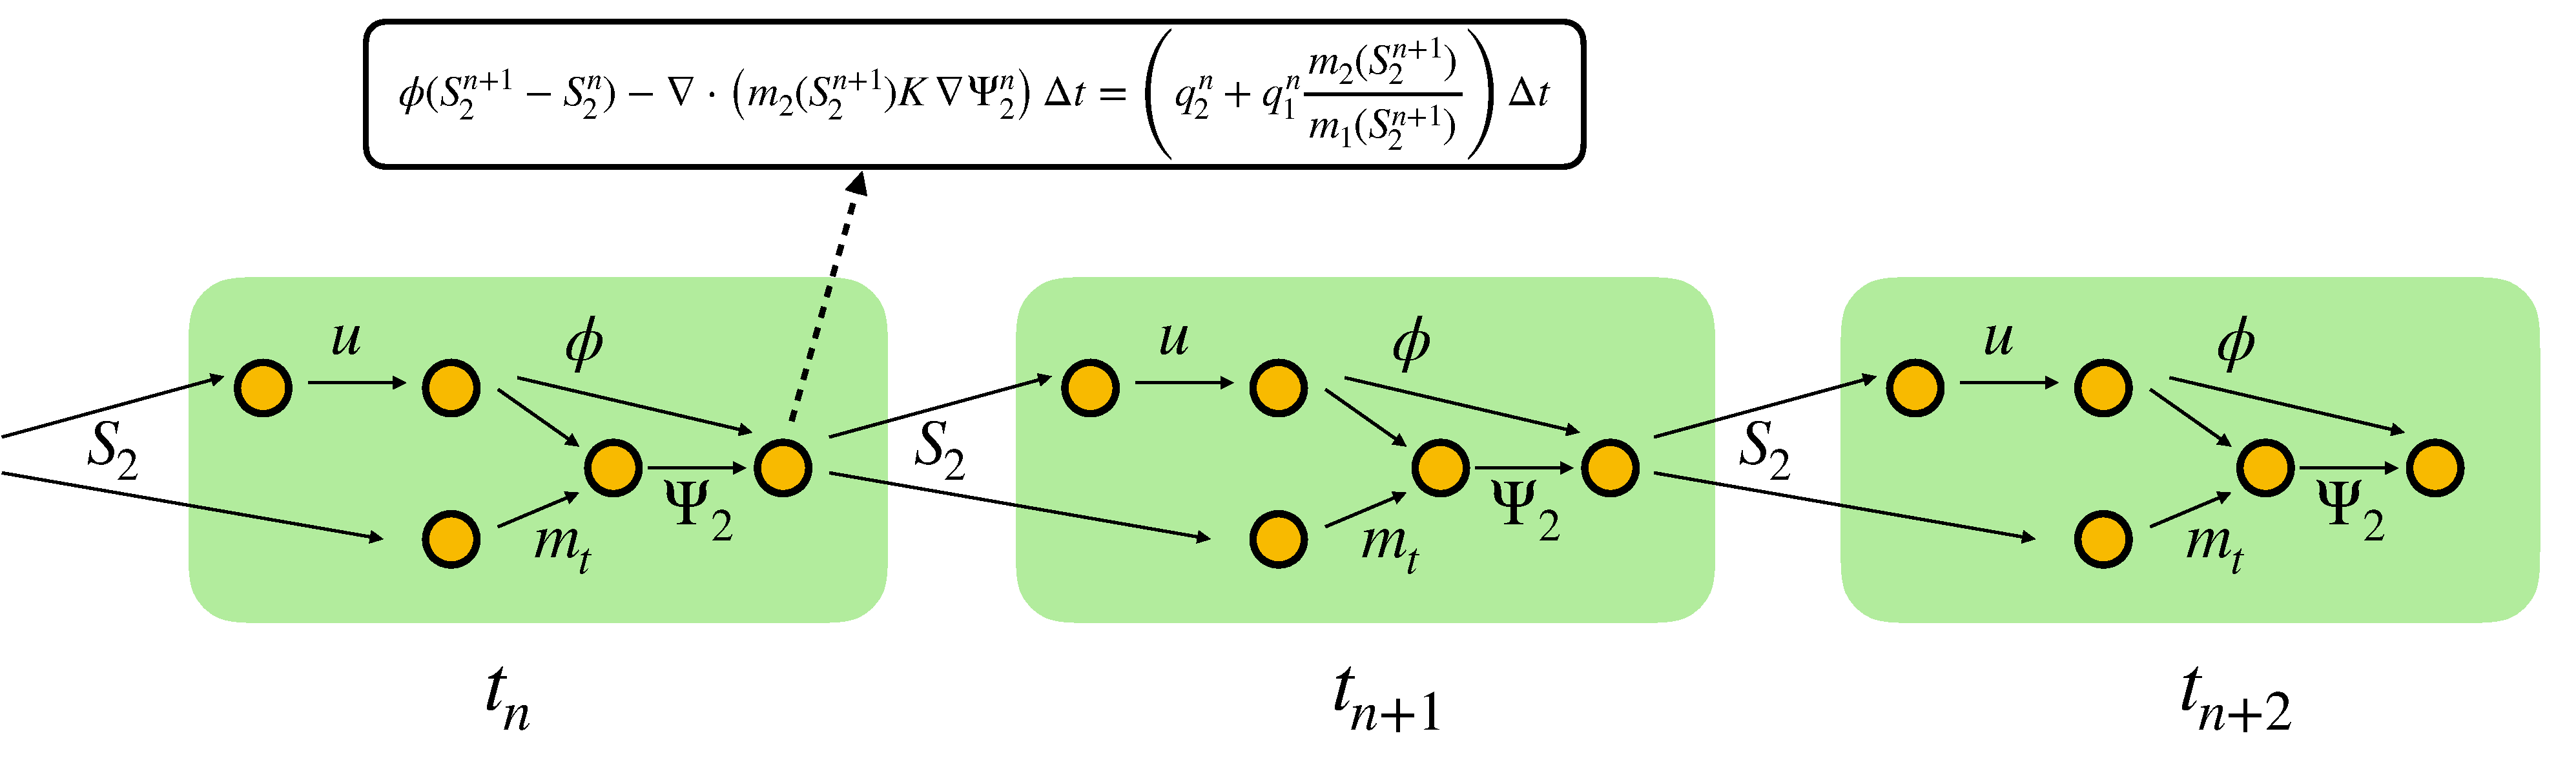
\includegraphics[width=1.0\textwidth]{figures/cgnum}
	\end{figure}
	
	
	
\end{frame}



\begin{frame}
	\frametitle{FEM/FVM on Structured Grids}
	\begin{itemize}
		\item Steady-state Navier-Stokes equation
		\begin{equation*}
		\begin{aligned}
		(\mathbf{u} \cdot \nabla) \mathbf{u} &=
		-\frac{1}{\rho} \nabla p + \nabla\cdot (\textcolor{red}{\nu(\mathbf{x})} \nabla \mathbf{u}) + \mathbf{g}\\
		\nabla \cdot \mathbf{u} &= 0
		\end{aligned}
		\end{equation*}
		
		\item Inverse problem are ubiquitous in fluid dynamics:
		
		\begin{figure}[hbt]
			\centering
			\includegraphics[width=0.4\textwidth]{figures/icepack}~
			\includegraphics[width=0.4\textwidth]{figures/covid}
			\caption{Left: electronic cooling; right: nasal drug delivery.}
		\end{figure}
		
	\end{itemize}
	
\end{frame}



\begin{frame}
	\frametitle{FEM/FVM on Structure Grids}
	
	\begin{figure}[hbt]
		\centering
		\includegraphics[width=0.49\textwidth]{figures/advertisement}~
		\includegraphics[width=0.49\textwidth]{figures/computational_graph}
	\end{figure}
\end{frame}



\begin{frame}
	\frametitle{FEM/FVM on Structure Grids}
	\begin{itemize}
		\item Data: $(u, v)$
		\item Unknown: $\nu(\mathbf{x})$ (represented by a deep neural network)
		\item Prediction: $p$ (absent in the training data) 
		\item The DNN provides regularization, which generalizes the estimation better!
	\end{itemize}
	\begin{figure}[hbt]
		\centering
		\includegraphics[width=1.0\textwidth]{figures/ns_result}~
	\end{figure}
\end{frame}


\begin{frame}
	\frametitle{A General Approach to Inverse Modeling}
	\begin{figure}[hbt]
  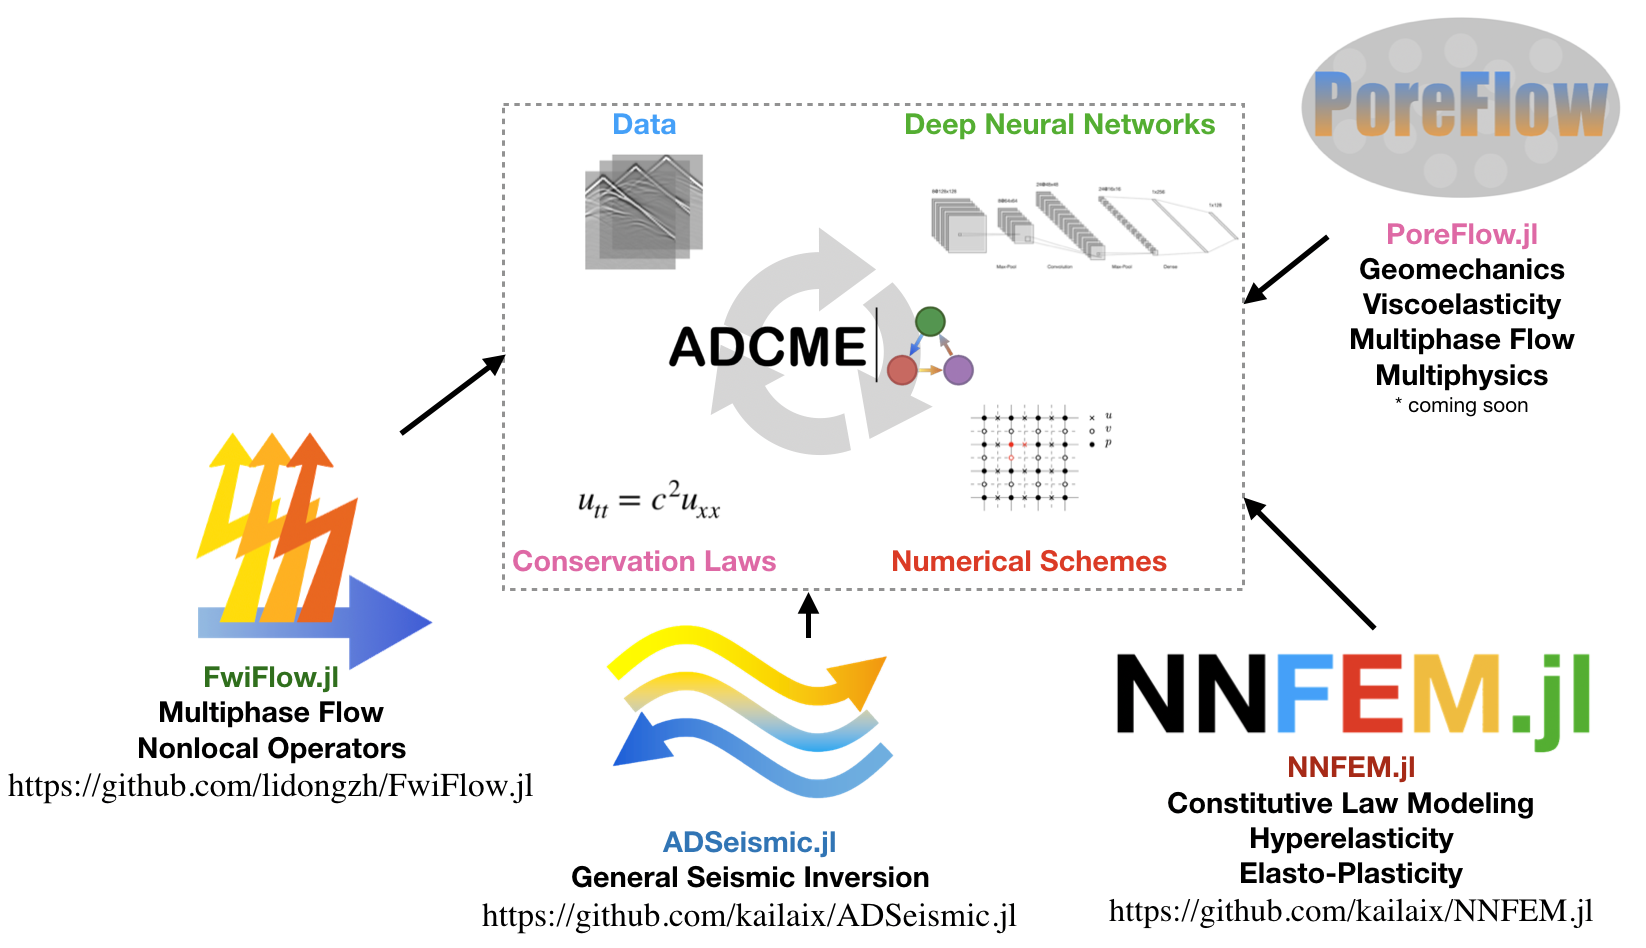
\includegraphics[width=1.0\textwidth]{figures/summary.png}
\end{figure}

\end{frame}




%}
%\usebackgroundtemplate{}
%----------------------------------------------------------------------------------------
%    PRESENTATION SLIDES
%----------------------------------------------------------------------------------------

%------------------------------------------------



\end{document} 